\chapter{Results} \label{results}


\section{Maximum Sound Frequency in Auscultation} \label{max-sound-freq}
In order optimise our system we determine what is the maximum sound frequency $f_{max}$ that it needs to measure. This frequency affects the design of the low pass filter and the sampling frequency needed for Analog to Digital Conversion. A lower $f_{max}$ results in a lower sampling frequency, which allows the microprocessor to carry out more computations per sample, and thus allows for higher order digital filters to be implemented. Higher order filters give greater flexibility in digitally manipulating the sound signal, and so would allow us to more accurately reproduce the sound characteristics of a conventional stethoscope.

An $f_{max}$ of 20kHz has been used in our design as this is the threshold of human hearing\cite[p.~163]{Stuart2011}, however it has been stated that the majority of heart and lung sounds occur at lower frequencies, within the range 37.5-1,000 Hz\cite{Abella1992}. In order to determine a lower limit on $f_{max}$ one hundred heart and lung sounds were analysed for their spectral content. Sound files were taken from an electronic resource used to train medical students in auscultation\cite{Coviello2014}, and three analyses were performed using MATLAB. 

The first analysis simply took a Fast Fourier Transform (FFT) of the sounds, summed the amplitudes and defined $f_{max}$ as the frequency at which this sum dropped below -80dB. In the second analysis all the sound signals were summed together, an FFT was performed on the resulting signal, and $f_{max}$ was defined to be the frequency at which the amplitude dropped below -80dB. In the third analysis the significant frequency components of each sound was calculated. Significant frequencies were defined as the range which contained 99.9\% of the signal energy, where energy is the sum of the squared FFT amplitudes. To calculate significant frequencies an iterative algorithm was used. The algorithm begins with a set that contains the signal's dominant frequency, it then adds to this set the next highest or lowest frequency, which ever has the larger FFT amplitude. The energy content of the set is compared with the energy of the sound, and the process continues until the set contains at least 99.9\% of the energy. Finally we took $f_{max}$ to be the largest frequency with at least one sound in which $f_{max}$ was considered significant. 

Analysis 1, 2, and 3 gave $f_{max}$ values 1.9kHz, 1.6kHz, and 4.0kHz respectively (Fig~\ref{fig:ausc_spectra}). If we use the most conservative result then our stethoscope needs to be able to measure and process frequencies up to at least 4.0kHz in order to capture all heart and lung sounds.

\begin{figure}[htb]
	\centering
	 \fbox{
		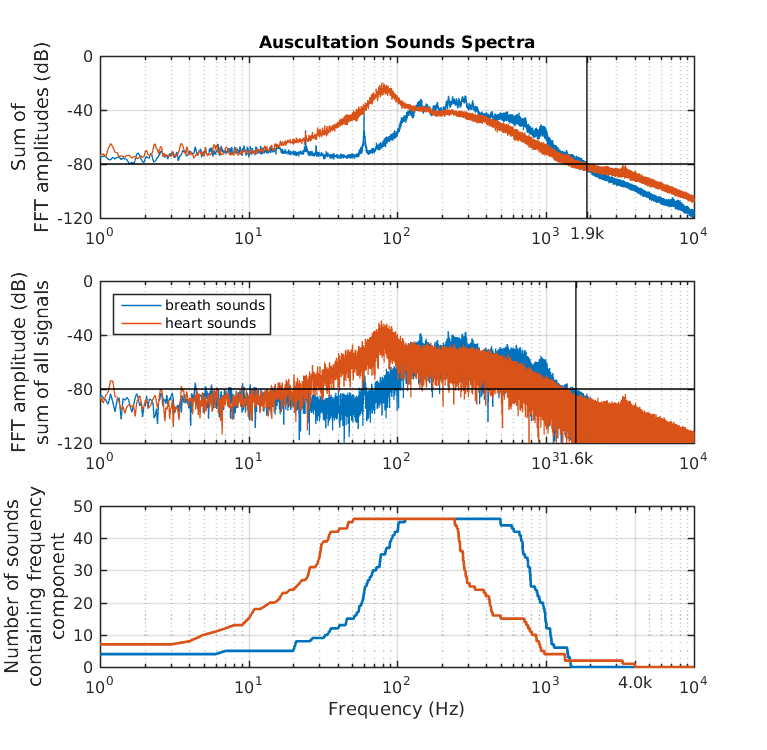
\includegraphics[width=135mm]{auscultation_spectra.png}
	 }
	\caption{Frequency spectra of auscultation sounds}
	\label{fig:ausc_spectra}
\end{figure}

\section{Frequency Response}
Freq response graphs

\section{Feedback} \label{feedback-freq}
Problem with feedback